\documentclass[aspectratio=169,11pt]{beamer}

\usepackage[utf8]{inputenc}
\usepackage[T1]{fontenc}
\usepackage[spanish,es-noquoting]{babel}
\usepackage{graphicx}
\usepackage{booktabs}
\usepackage{amsmath}

\usetheme{metropolis}
\metroset{numbering=fraction, progressbar=frametitle, block=fill}

\definecolor{uvgazul}{RGB}{31,58,120}
\setbeamercolor{frametitle}{bg=uvgazul}
\setbeamercolor{progress bar}{fg=uvgazul!60}
\setbeamercolor{alerted text}{fg=uvgazul}

\graphicspath{{../informe/figuras/}}

\title{Análisis Exploratorio}
\subtitle{Reto 18: Hackeando el cuerpo humano \\ HuBMAP: segmentación de unidades funcionales de tejido}
\author{Iris Ayala (23965) \and Jonatan Díaz (23837) \and Anggie Quezada (23643)}
\institute{Universidad del Valle de Guatemala \\ CC3084 Data Science, Semestre II, 2026}
\date{\today}

\begin{document}

\maketitle

%----------------------------------------------------------------------
\begin{frame}{Agenda}
  \setbeamertemplate{section in toc}[sections numbered]
  \tableofcontents
\end{frame}

%======================================================================
\section{El problema}
%======================================================================

\begin{frame}{¿Qué es una unidad funcional de tejido?}
  \begin{columns}[T]
    \begin{column}{0.56\textwidth}
      Una \alert{FTU} es un grupo pequeño de células organizadas alrededor de un vaso sanguíneo que
      cumplen juntas una función dentro del órgano.

      \vspace{0.5em}
      El reto cubre \alert{cinco órganos}, y en cada uno la FTU se ve distinta:

      \begin{itemize}
        \item Riñón $\rightarrow$ glomérulos
        \item Intestino grueso $\rightarrow$ criptas
        \item Próstata $\rightarrow$ unidades glandulares
        \item Bazo y pulmón $\rightarrow$ estructuras propias
      \end{itemize}
    \end{column}
    \begin{column}{0.42\textwidth}
      \begin{block}{Contexto}
        HuBMAP quiere mapear el cuerpo humano a nivel de célula.

        \vspace{0.4em}
        Las muestras se tiñen con \alert{PAS}, que resalta membranas basales y estructuras
        glandulares. De ahí el tono rosado y morado.
      \end{block}
    \end{column}
  \end{columns}
\end{frame}

\begin{frame}{Situación problemática}
  Hoy las FTU las marca un \alert{patólogo a mano}, al microscopio.

  \vspace{1em}
  \begin{columns}[T]
    \begin{column}{0.31\textwidth}
      \begin{block}{Lento}
        Imagen por imagen, estructura por estructura.
      \end{block}
    \end{column}
    \begin{column}{0.31\textwidth}
      \begin{block}{Subjetivo}
        Depende de la experiencia de quien lo hace.
      \end{block}
    \end{column}
    \begin{column}{0.31\textwidth}
      \begin{block}{No escala}
        Imposible con miles de imágenes de distintos órganos.
      \end{block}
    \end{column}
  \end{columns}

  \vspace{1.2em}
  Y encima, muestras del mismo órgano preparadas en \alert{laboratorios distintos no se ven igual}.
\end{frame}

\begin{frame}{Problema científico y objetivos}
  \begin{alertblock}{Pregunta de investigación}
    A partir de una imagen de tejido, ¿se puede entrenar un modelo que marque con precisión dónde
    están las unidades funcionales de tejido, sin importar el órgano ni la fuente de la muestra?
  \end{alertblock}

  \vspace{0.6em}
  \textbf{Objetivo general.} Explorar y describir los datos para entender cómo están compuestas las
  imágenes y las variables que las acompañan, como base para una futura solución de segmentación.

  \vspace{0.4em}
  \textbf{Objetivos específicos.}
  \begin{enumerate}
    \item Describir las variables numéricas y categóricas y detectar diferencias entre grupos.
    \item Analizar cómo se relacionan órgano, fuente, edad y sexo.
    \item Cuantificar el área que ocupa la FTU y comparar su distribución entre órganos.
  \end{enumerate}
\end{frame}

%======================================================================
\section{Los datos}
%======================================================================

\begin{frame}{Qué tenemos}
  \begin{columns}[T]
    \begin{column}{0.46\textwidth}
      \begin{block}{\texttt{train.csv}}
        \begin{itemize}
          \item \alert{351} observaciones, una por imagen
          \item \alert{10} variables
          \item \alert{0} valores nulos
          \item \alert{0} filas duplicadas
        \end{itemize}
      \end{block}
      \vspace{0.3em}
      Limpieza aplicada: convertir \texttt{organ}, \texttt{data\_source} y \texttt{sex} a tipo
      categórico. Nada más hizo falta.
    \end{column}
    \begin{column}{0.5\textwidth}
      \small
      \begin{tabular}{ll}
        \toprule
        \textbf{Variable} & \textbf{Tipo} \\
        \midrule
        \texttt{id}                & identificador \\
        \texttt{organ}             & categórica \\
        \texttt{data\_source}      & categórica \\
        \texttt{sex}               & categórica \\
        \texttt{img\_height/width} & numérica \\
        \texttt{pixel\_size}       & numérica \\
        \texttt{tissue\_thickness} & numérica \\
        \texttt{age}               & numérica \\
        \texttt{rle}               & texto (máscara) \\
        \bottomrule
      \end{tabular}
    \end{column}
  \end{columns}
\end{frame}

\begin{frame}{La columna \texttt{rle}: dónde está la información real}
  La máscara de la FTU no viene como imagen, viene comprimida en
  \alert{run-length encoding}: pares de (posición inicial, longitud).

  \vspace{0.8em}
  \begin{exampleblock}{Por qué importa}
    Guardar una máscara de $3000 \times 3000$ píxeles como matriz sería inviable dentro de una celda
    de texto. El rle la reduce a unos miles de caracteres.
  \end{exampleblock}

  \vspace{0.8em}
  De ahí construimos la variable que de verdad describe el problema:

  \begin{equation*}
    \texttt{mask\_frac} =
    \frac{\text{píxeles marcados como FTU}}{\texttt{img\_height} \times \texttt{img\_width}}
  \end{equation*}

  Basta con \alert{sumar las longitudes}, sin reconstruir la máscara completa.
\end{frame}

%======================================================================
\section{Análisis exploratorio}
%======================================================================

\begin{frame}{Variables univariadas}
  \begin{figure}
    \centering
    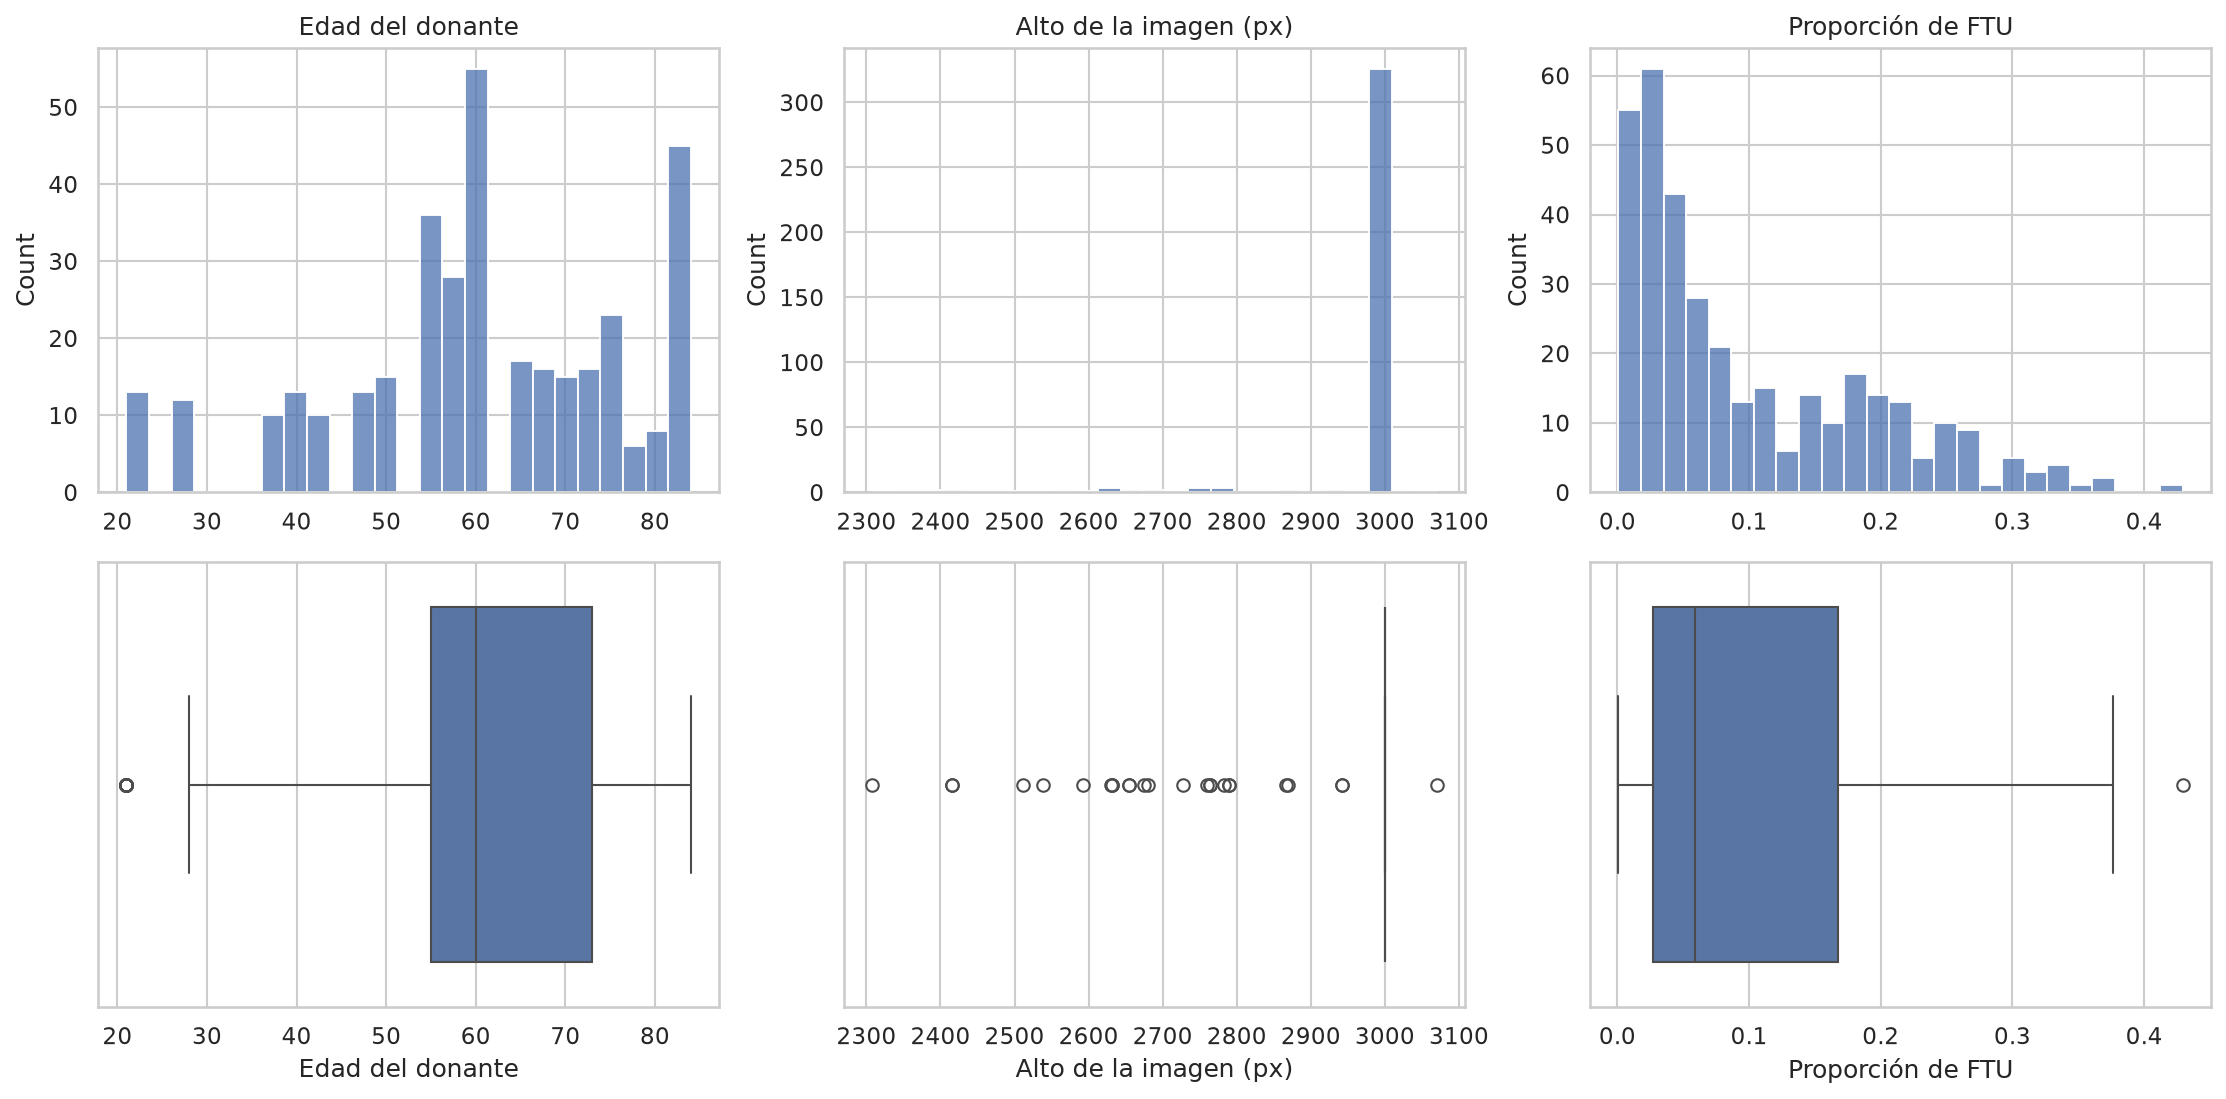
\includegraphics[width=0.92\textwidth]{univariadas.png}
  \end{figure}
  \small
  Edad de 21 a 84 años, mediana 60. Casi todas las imágenes son de $3000 \times 3000$. La proporción
  de FTU está \alert{sesgada a la derecha}: mediana de apenas 0.059.
\end{frame}

\begin{frame}{Variables categóricas}
  \begin{figure}
    \centering
    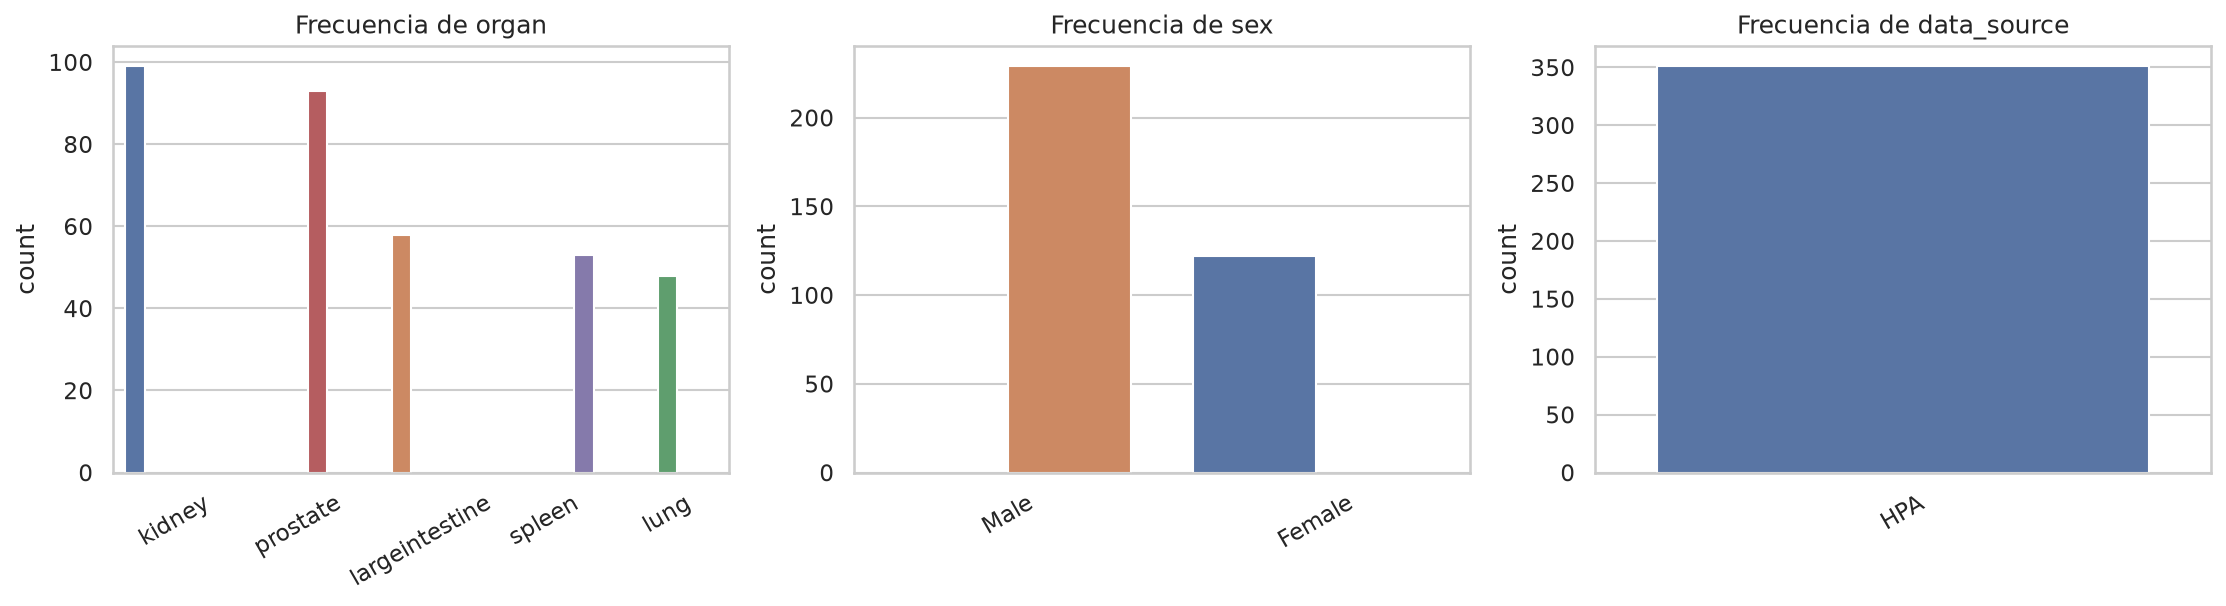
\includegraphics[width=0.95\textwidth]{categoricas.png}
  \end{figure}
  \small
  Desbalance por órgano (99 riñones contra 48 pulmones) y por sexo (229 hombres contra 122 mujeres).
  Y \texttt{data\_source} tiene \alert{una sola barra}. Volvemos a eso en un momento.
\end{frame}

\begin{frame}{Cruces por órgano}
  \begin{figure}
    \centering
    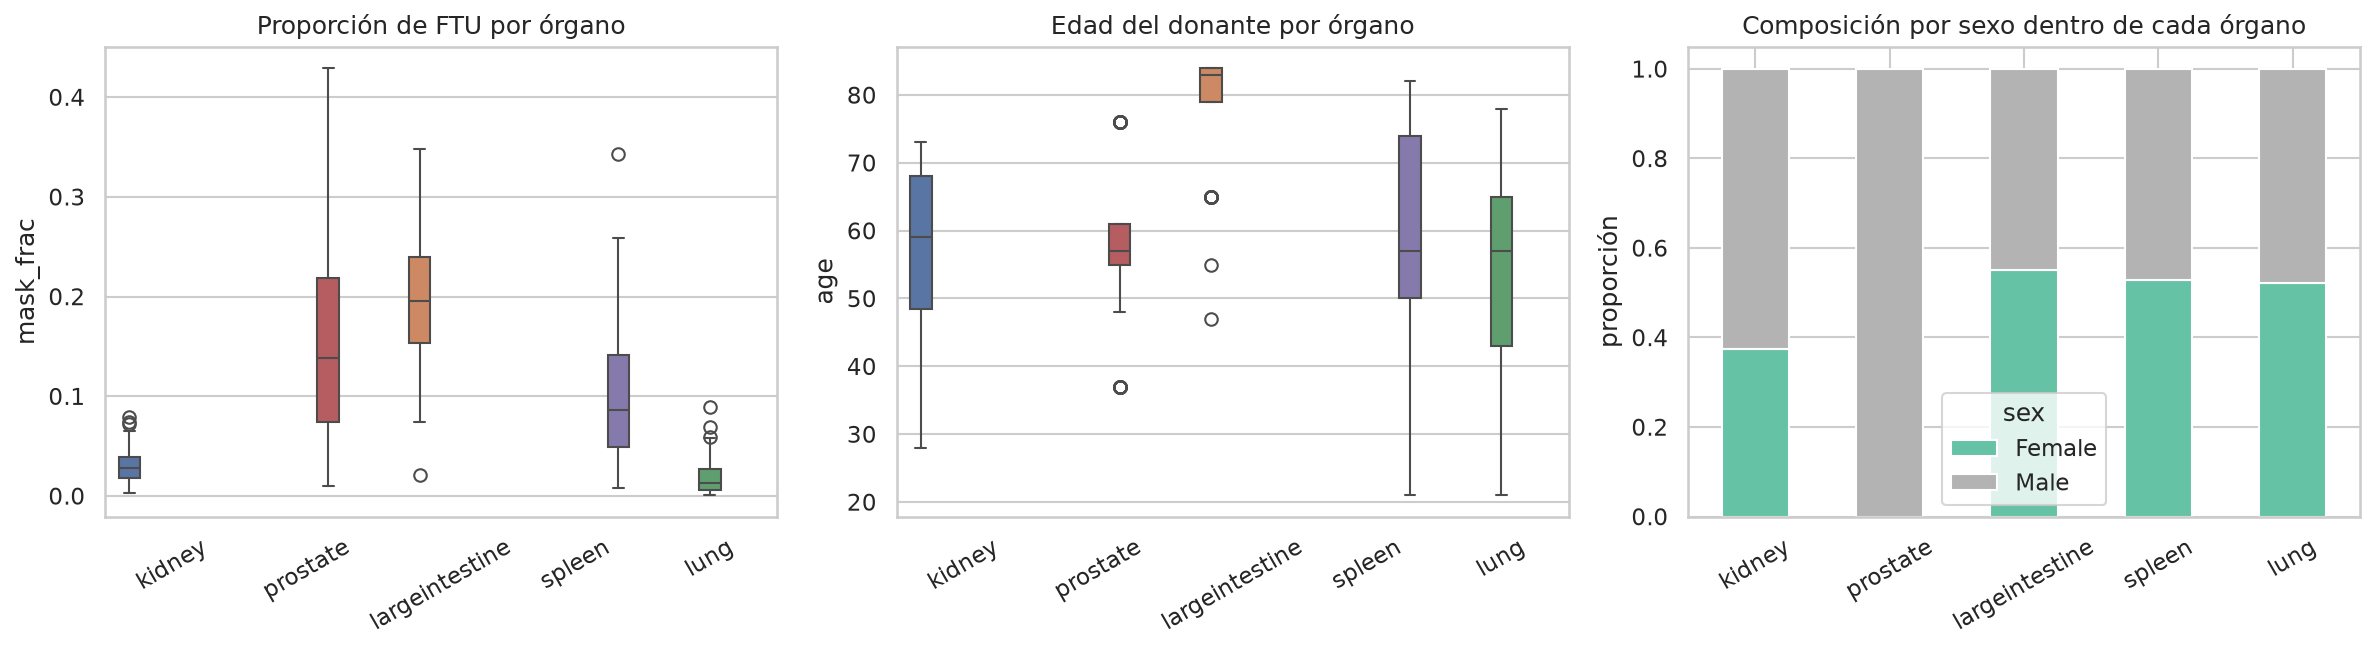
\includegraphics[width=0.95\textwidth]{cruces.png}
  \end{figure}
  \small
  Próstata es 100\,\% masculino, lo cual es biología y no un error. Intestino grueso tiene una edad
  mediana de 83 años contra 57 a 59 del resto: \alert{órgano y edad no son independientes}.
\end{frame}

\begin{frame}{Outliers: cuidado con aplicarlos a ciegas}
  \begin{columns}[T]
    \begin{column}{0.48\textwidth}
      \begin{block}{\texttt{age}: 13 outliers}
        Todos con valor 21 años. Pero 21 cae dentro del rango normal de pulmón y bazo.

        \vspace{0.4em}
        Son atípicos \alert{solo si se ignora el órgano}.
      \end{block}
    \end{column}
    \begin{column}{0.48\textwidth}
      \begin{block}{\texttt{img\_height}: 25 outliers}
        El 75\,\% de las imágenes mide exactamente 3000 px, así que el rango intercuartílico es
        \alert{cero} y el método marca todo lo que no sea 3000.

        \vspace{0.4em}
        La variable es casi binaria, no continua.
      \end{block}
    \end{column}
  \end{columns}

  \vspace{1em}
  En ambos casos se documenta el hallazgo y \alert{no se elimina nada}. Sobre valores faltantes: no
  hay ninguno en las 351 filas.
\end{frame}

%======================================================================
\section{Hallazgos}
%======================================================================

\begin{frame}{Hallazgo 1: hay variables que no dicen nada}
  \begin{columns}[T]
    \begin{column}{0.52\textwidth}
      \begin{alertblock}{Constantes en las 351 filas}
        \texttt{pixel\_size} $= 0.4$

        \texttt{tissue\_thickness} $= 4.0$
      \end{alertblock}
      Varianza cero. Por eso aparecen como \texttt{NaN} en la matriz de correlación: el coeficiente
      de Pearson implica dividir entre la desviación estándar.

      \vspace{0.5em}
      \alert{No es un bug del código.}
    \end{column}
    \begin{column}{0.44\textwidth}
      \begin{block}{Y además}
        \texttt{img\_height} $=$ \texttt{img\_width} en todas las filas: las imágenes son cuadradas.

        \vspace{0.4em}
        326 de 351 son de $3000 \times 3000$.
      \end{block}
      \vspace{0.3em}
      De las variables tabulares, solo \texttt{organ}, \texttt{sex}, \texttt{age} y la derivada de
      \texttt{rle} tienen información real.
    \end{column}
  \end{columns}
\end{frame}

\begin{frame}{Hallazgo 2: la FTU no ocupa lo mismo en cada órgano}
  \begin{columns}[T]
    \begin{column}{0.6\textwidth}
      \begin{figure}
        \centering
        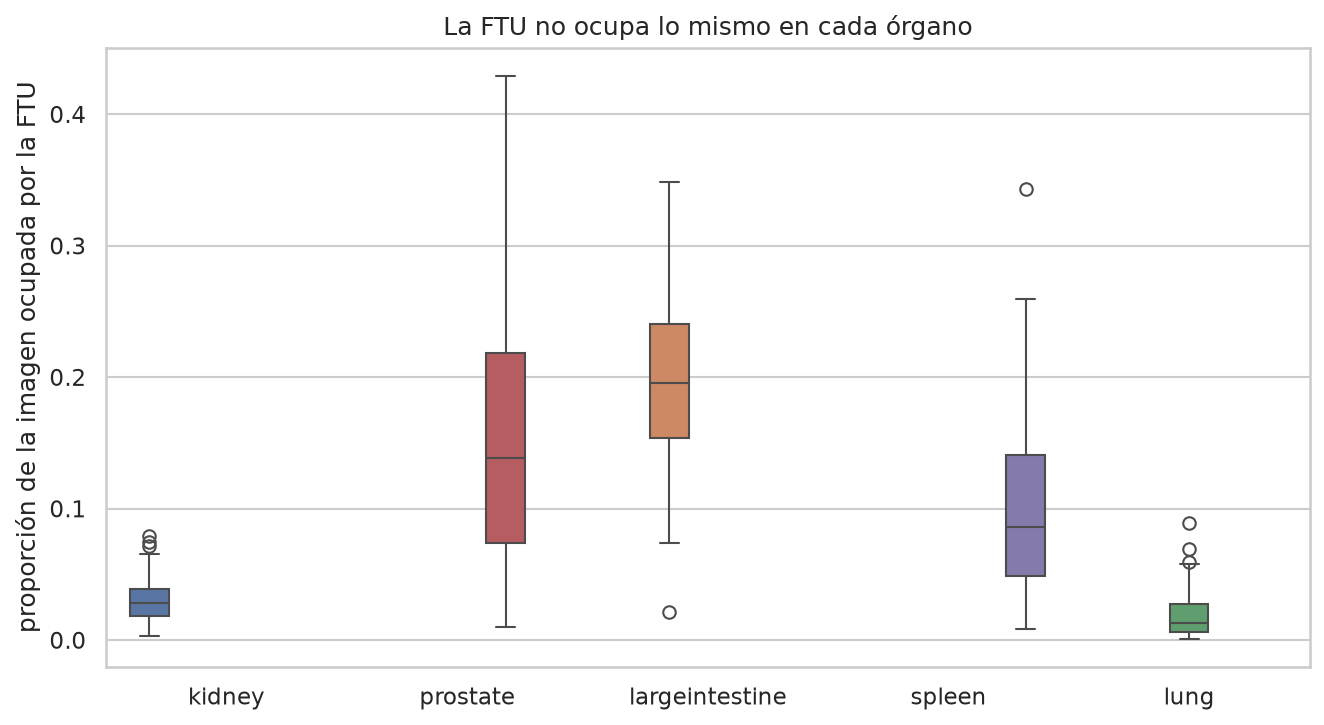
\includegraphics[width=\textwidth]{ftu_por_organo.png}
      \end{figure}
    \end{column}
    \begin{column}{0.38\textwidth}
      \small
      \begin{tabular}{lr}
        \toprule
        \textbf{Órgano} & \textbf{mediana} \\
        \midrule
        largeintestine & 19.6\,\% \\
        prostate       & 13.8\,\% \\
        spleen         &  8.6\,\% \\
        kidney         &  2.8\,\% \\
        lung           &  1.3\,\% \\
        \midrule
        \textbf{global} & \textbf{5.9\,\%} \\
        \bottomrule
      \end{tabular}

      \vspace{0.8em}
      \alert{Quince veces} de diferencia entre intestino grueso y pulmón.

      \vspace{0.5em}
      Encontrar la FTU no es el mismo problema en cada órgano.
    \end{column}
  \end{columns}
\end{frame}

\begin{frame}{Hallazgo 3: una correlación que engaña}
  \begin{figure}
    \centering
    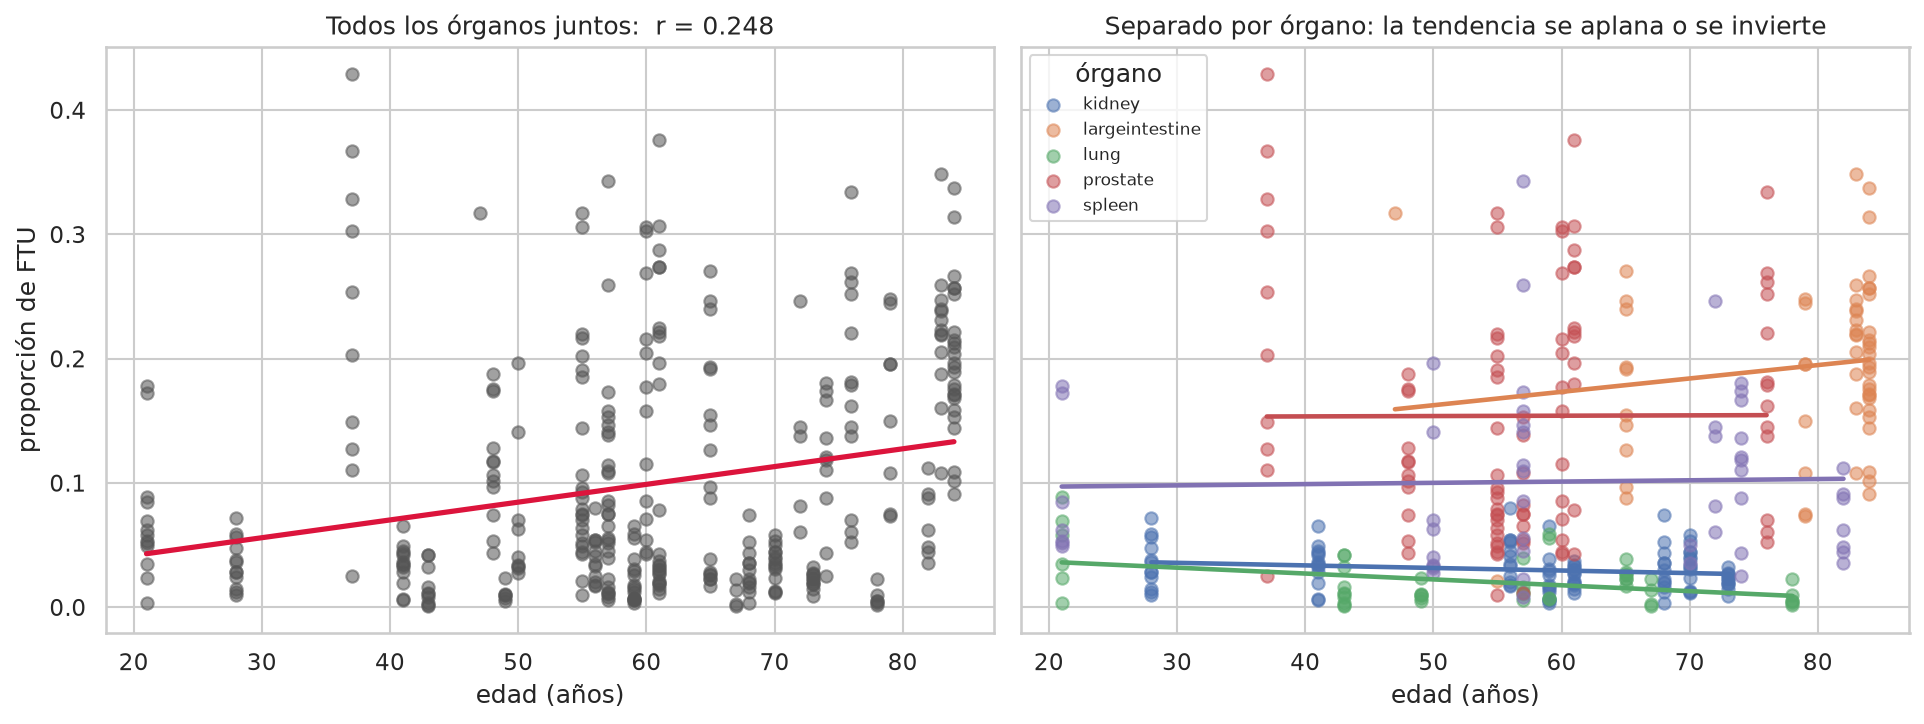
\includegraphics[width=0.93\textwidth]{simpson.png}
  \end{figure}
\end{frame}

\begin{frame}{Hallazgo 3: paradoja de Simpson}
  \begin{columns}[T]
    \begin{column}{0.42\textwidth}
      \small
      \begin{tabular}{lr}
        \toprule
        \textbf{Grupo} & \textbf{r (edad, FTU)} \\
        \midrule
        \textbf{Global} & \textbf{$+0.248$} \\
        \midrule
        kidney          & $-0.178$ \\
        largeintestine  & $+0.139$ \\
        lung            & $-0.396$ \\
        prostate        & $+0.003$ \\
        spleen          & $+0.028$ \\
        \bottomrule
      \end{tabular}
    \end{column}
    \begin{column}{0.55\textwidth}
      La correlación global \alert{no mide edad contra tamaño de FTU}. Mide el órgano disfrazado.

      \vspace{0.6em}
      Intestino grueso tiene a la vez los donantes más viejos (mediana 83 años) y las FTU más
      grandes (19.6\,\%). Al mezclar todo, ese grupo arrastra la correlación hacia arriba.

      \vspace{0.6em}
      \begin{alertblock}{Implicación}
        Cualquier correlación calculada sobre este conjunto \alert{sin estratificar por órgano} es
        poco confiable.
      \end{alertblock}
    \end{column}
  \end{columns}
\end{frame}

\begin{frame}{Hallazgo 4: el desbalance está en varios ejes a la vez}
  \begin{columns}[T]
    \begin{column}{0.31\textwidth}
      \begin{block}{Por órgano}
        99 riñones \\ contra \\ 48 pulmones
      \end{block}
    \end{column}
    \begin{column}{0.31\textwidth}
      \begin{block}{Por sexo}
        229 hombres \\ contra \\ 122 mujeres
      \end{block}
    \end{column}
    \begin{column}{0.31\textwidth}
      \begin{block}{Por edad}
        Concentrado \\ entre \\ 55 y 73 años
      \end{block}
    \end{column}
  \end{columns}

  \vspace{1.2em}
  Y no son independientes entre sí: los 93 casos de próstata son todos masculinos, e intestino
  grueso concentra a los donantes de mayor edad.

  \vspace{0.8em}
  \alert{El desbalance de un eje se filtra en los otros.}
\end{frame}

\begin{frame}{Hallazgo 5: la dificultad del reto no está en los datos}
  \begin{alertblock}{Las 351 filas tienen \texttt{data\_source = HPA}}
    No hay ni una sola observación de HuBMAP en \texttt{train.csv}.
  \end{alertblock}

  \vspace{0.8em}
  Las muestras de HuBMAP quedan del lado del conjunto de prueba de la competencia.

  \vspace{0.8em}
  Pero la dificultad central del reto es justamente que el modelo funcione con muestras preparadas
  en \alert{laboratorios distintos}.

  \vspace{0.8em}
  \begin{exampleblock}{Conclusión}
    La variabilidad que el modelo tiene que superar \alert{no se puede observar ni medir} dentro de
    los datos de entrenamiento.
  \end{exampleblock}
\end{frame}

%======================================================================
\section{Conclusiones}
%======================================================================

\begin{frame}{Siguientes pasos}
  \begin{enumerate}
    \item \textbf{Descartar las variables constantes.} \texttt{pixel\_size} y
          \texttt{tissue\_thickness} no discriminan nada.

    \item \textbf{Tratar el problema como segmentación desbalanceada.} Con 5.9\,\% de píxeles
          positivos, predecir fondo en toda la imagen daría más del 94\,\% de exactitud por píxel y
          sería inútil. Usar Dice o IoU, no exactitud.

    \item \textbf{Validar por órgano, no solo en global.} El promedio esconde que pulmón y riñón son
          mucho más difíciles.

    \item \textbf{Estratificar todo análisis por órgano.} Lo demostró la paradoja de Simpson.

    \item \textbf{Apoyarse en aumentación de color y tinción.} Es la única vía para simular la
          variabilidad entre fuentes que el entrenamiento no contiene.
  \end{enumerate}
\end{frame}

\begin{frame}[standout]
  Gracias

  \vspace{1em}
  \small\normalfont
  \texttt{github.com/AleWWH1104/proyecto2-data}
\end{frame}

\end{document}
